\chapter{Podsumowanie i wnioski}\label{chap:podsumowanie_i_wnioski}
Celem niniejszej pracy było przeprowadzenie analizy porówawczej zróżnicowanej grupy dostępnych neuronowych wizyjnych algorytmów percepcji głębi. W szczególności skupiono się na obiektywnej ocenie ich dokładności, wydajności czasowej, ogólnej efektywności w różnych zastosowaniach oraz wymagań systemowych.

W ramach analizy porównano sześć algorytmów wybranych pod kątem wyników osiąganych w publicznie dostępnych zestawieniach, architektury oraz metody ich uczenia. W celu wykonania rzetelnej analizy wykorzystany został szereg metryk, takich jak pierwiastek ze średniego błądu kwadratowego czy średni bezwzględny błąd procentowy.

W bieżącym rozdziale zawarte jest podsumowanie dokonanej analizy porównawczej oraz wnioski z niej płynące. Przedstawione zostaną kluczowe spostrzeżenia, wskazujące na mocne i słabe strony poszczególnych algorytmów, oraz rekomendacje dotyczące ich zastosowań w praktyce.

\section{Podsumowanie wyników}
W celu usystematyzowania i podsumowania wyników uzyskanych przez algorytmy zostało przygotowane zestawienie średnich wartości uzyskanych na wszystkich zestawach danych (tabela \ref{table:metrics}). Takie zestawienie pozwala na przejrzyste porównanie efektywności algorytmów i wyciągnięcie jednoznacznych wniosków dotyczących ich wydajności i dokładności w założonym środowisku testowym. Kolorem zielonym oznaczone zostały najlepsze wyniki, kolorem czerwonym najgorsze.

\begin{table}[H]
    \centering
    \caption{Średnie wartości wyników uzyskanych przez algorytmy.}
    \vspace{0.1cm}
    \resizebox{\textwidth}{!}{%
        \begin{tabular}{|l|c|c|c|c|c|c|}
        \hline
        \textbf{Metryka} & \textbf{Metric3D} & \textbf{DepthAnythingV2} & \textbf{MetaPrompt-SD} & \textbf{SQLdepth} & \textbf{AdelaiDepth} & \textbf{GCNDepth} \\
        \hline
        $\delta < 1.25$ & \textcolor{OliveGreen}{0,883} & 0,584 & 0,389 & 0,266 & 0,306 & \textcolor{BrickRed}{0,245} \\
        $\delta < 1,25^2$ & \textcolor{OliveGreen}{0,968} & 0,857 & 0,586 & 0,376 & 0,506 & \textcolor{BrickRed}{0,348} \\
        $\delta < 1,25^3$ & \textcolor{OliveGreen}{0,983} & 0,939 & 0,740 & 0,511 & 0,627 & \textcolor{BrickRed}{0,480} \\
        \hline
        AbsRel & \textcolor{OliveGreen}{11,75} & 29,78 & 62,30 & 125,68 & \textcolor{BrickRed}{218,04} & 141,14 \\
        RMSE & 4,655 & \textcolor{OliveGreen}{3,358} & 3,844 & 6,276 & \textcolor{BrickRed}{42,146} & 7,265 \\
        \hline
        czas (s) & \textcolor{BrickRed}{3,628} & 1,487 & 2,038 & 0,777 & 0,728 & \textcolor{OliveGreen}{0,449} \\
        \hline
        \end{tabular}%
    }
\label{table:metrics}
\end{table}

\section{Interpretacja wyników}
\subsection{Dokładność estymacji}
W aspekcie dokładności estymacji zdecydowanym liderem jest algorytm \textbf{Metric3D} osiągający najlepszy wynik w większości metrykach dokładności predykcji. Jedynie średnia wartości pierwiastków błędu średniokwadratowego (RMSE) tego algorytmu jest nieoczekiwanie wyższa w porównaniu do pozostałych wiodących algorytmów, jest to jednak skutkiem wysokiego wyniku uzyskanego na syntetycznym zbiorze Taskonomy (21.322), spowodowanym dużą ilością scen zawierających przeszklenia. Algorytm Metric3D bowiem w wielu przypadkach estymuje odległość do przeszklenia, podczas gdy zestaw Taskonomy zawiera głębię do obiektu za przeszkleniem (rys. \ref{fig:metric3d-taskonomy}). Model Metric3D jest ponadprzeciętnie dokładny w dużej mierze dzięki implementacji wykorzystania informacji dotyczącej długości ogniskowej kamery. Pomijając etap wykorzystujący rzeczoną informację, algorytm ten estymuje poprawnie głębię relatywną, jest ona jednak przesunięta względem wartości rzeczywistych. Funkcjonuje poprawnie na scenach zewnętrznych oraz wewnętrznych co świadczy o bardzo wysokiej generalizacji i uniwersalności tego modelu.
\begin{figure}[H]
    \centering
    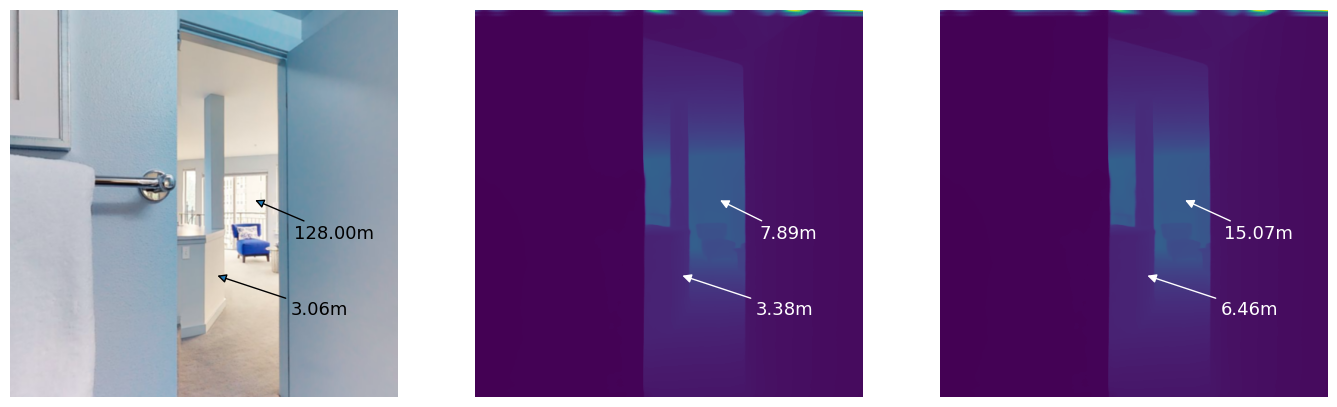
\includegraphics[width=1\textwidth]{49.jpg}
    \caption{Wizualizacja estymacji algorytmu Metric3D na obrazie z zestawu Taskonomy.}
    \label{fig:metric3d-taskonomy}
\end{figure}

Następne miejsce pod kątem dokładności zajął algorytm \textbf{Depth Anything V2} uczony metodą częściowo nadzorowaną na największej ilości obrazów spośród wszystkich analizowanych algorytmów. Należy jednak wziąć pod uwagę fakt, że model ten do funkcjonowania nie wymaga żadnych dodatkowych informacji poza obrazem wejściowym w przeciwieństwie do Metric3D. Rozwiązanie Depth Anything V2 wykazuje wysoką efektywność zarówno na scenach zewnętrznych jak i wewnętrznych (rys. \ref{fig:depthanything-stray}), jest to jednak niewątpliwie zasługa odrębnych wag modelu do obu rodzajów scen. Metoda Depth Anything V2 osiągnęła najniższą wartość RMSE spośród wszystkich analizowanych modeli.
\begin{figure}[H]
    \centering
    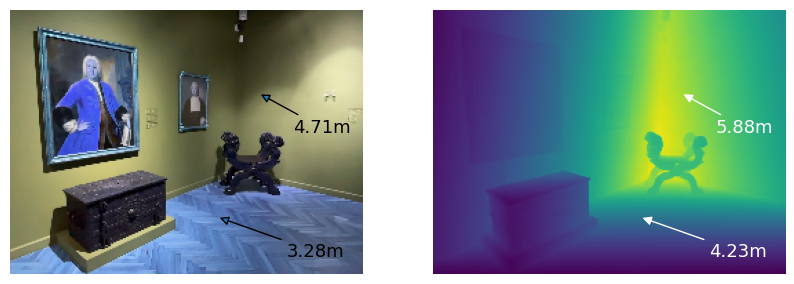
\includegraphics[width=1\textwidth]{50.jpg}
    \caption{Wizualizacja estymacji algorytmu Depth Anything V2 na obrazie z zestawu autorskiego.}
    \label{fig:depthanything-stray}
\end{figure}

Trzecią najdokładniejszą metodą jest \textbf{MetaPrompt-SD}. Odbiega ona jednak w sposób zauważalny od najdokładniejszej metody - wykazuje ponad pięciokrotnie gorszy średni wynik AbsRel. Najgorszy rezultat przyniósł test przeprowadzony na obu podzbiorach DIODE (rys. \ref{fig:metaprompt-diode}). Może to być spowodowane wysokim stopniem skomplikowania scen w tym zbiorze. Model funkcjonuje równie efektywnie niezależnie od zlokalizowania scen. Metoda MetaPrompt-SD została nauczona jedynie na dwóch zbiorach - NYUv2 oraz KITTI. Pomimo to osiągnęła najlepszy wynik AbsRel na syntetycznym zbiorze scen wewnętrznych Taskonomy (rys. \ref{fig:metaprompt-taskonomy}).
\begin{figure}[H]
    \centering
    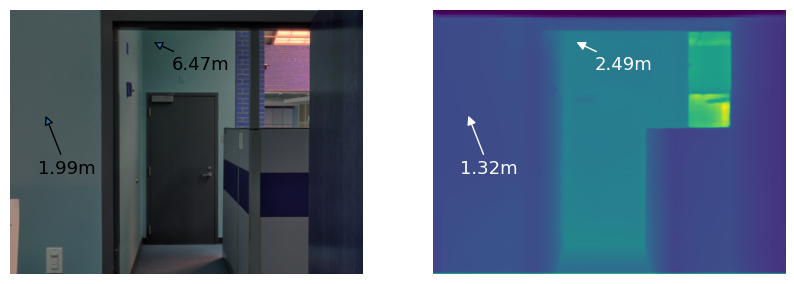
\includegraphics[width=1\textwidth]{51.jpg}
    \caption{Wizualizacja estymacji algorytmu MetaPrompt-SD na obrazie z zestawu DIODE.}
    \label{fig:metaprompt-diode}
\end{figure}
\begin{figure}[H]
    \centering
    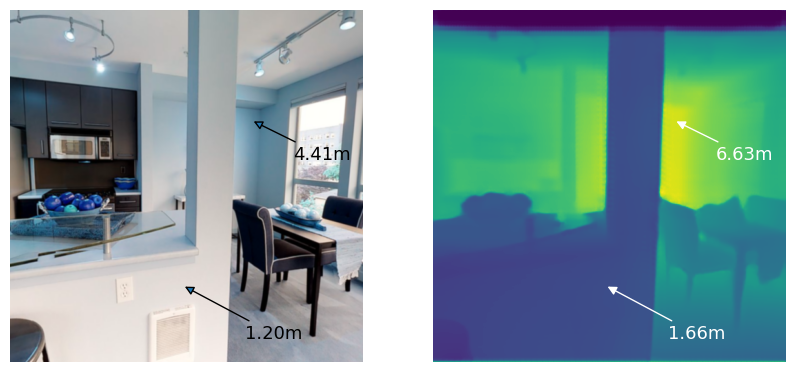
\includegraphics[width=1\textwidth]{52.jpg}
    \caption{Wizualizacja estymacji algorytmu MetaPrompt-SD na obrazie z zestawu Taskonomy.}
    \label{fig:metaprompt-taskonomy}
\end{figure}

Algorytmy \textbf{GCNDepth} (rys. \ref{fig:GCNDepth-KITTI}) oraz \textbf{SQLdepth} (rys. \ref{fig:SQLdepth-KITTI}) wykazują bardzo niskie zdolności generalizacji. Pomimo różnic w architekturze, obie metody nauczone na jednym zestawie - KITTI - jedynie na nim oraz jego wirtualnym odpowiedniku (Virtual KITTI 2) osiągnęły średni bezwzględny błąd procentowy poniżej 20\%. Z tego względu należy je rozpatrywać jedynie w kontekście charakterystyki scen przedstawionych we wsponianych zestawach, czyli głównie scen prezentujących miejski ruch uliczny.
\begin{figure}[H]
    \centering
    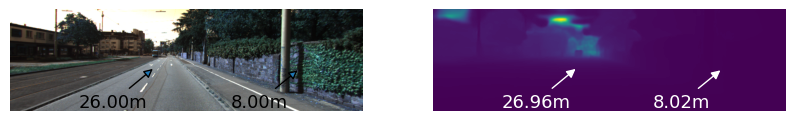
\includegraphics[width=1\textwidth]{54.jpg}
    \caption{Wizualizacja estymacji algorytmu GCNDepth na obrazie z zestawu KITTI.}
    \label{fig:GCNDepth-KITTI}
\end{figure}
\begin{figure}[H]
    \centering
    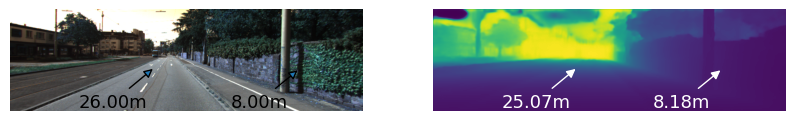
\includegraphics[width=1\textwidth]{55.jpg}
    \caption{Wizualizacja estymacji algorytmu SQLdepth na obrazie z zestawu KITTI.}
    \label{fig:SQLdepth-KITTI}
\end{figure}

Najgorszy wynik w założonym środowisku testowym uzyskał algorytm \textbf{AdelaiDepth}. Pomimo że został nauczony na zbiorze Taskonomy uzyskał na nim najgorszy wynik AbsRel spośród analizowanych algorytmów. Może to świadczyć o niewielkim udziale tego zbioru w procesie uczenia. Model AdelaiDepth osiąga akceptowalne rezultaty jedynie na scenach wewnętrznych (rys. \ref{fig:adelaidepth-stray}).
\begin{figure}[H]
    \centering
    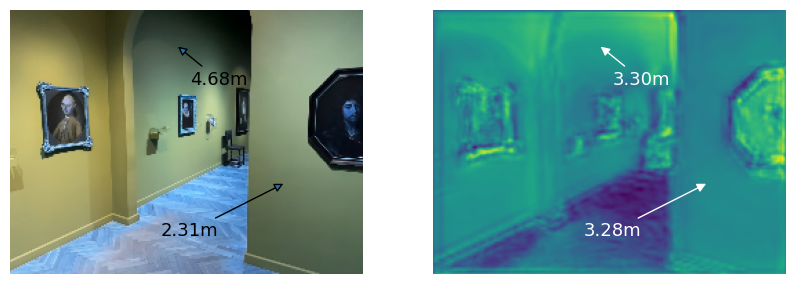
\includegraphics[width=1\textwidth]{53.jpg}
    \caption{Wizualizacja estymacji algorytmu AdelaiDepth na obrazie z zestawu autorskiego.}
    \label{fig:adelaidepth-stray}
\end{figure}

Wizualizacje dla każdej z porównywanych metod na wszystkich wymienionych w tym podrozdziale zestawach zostały umieszczone w załączniku do niniejszej pracy (tabele \ref{tab:vis-beg} - \ref{tab:vis-end}).


\subsection{Wydajność czasowa}
Analiza wydajności czasowej stanowi kluczową kwestię dla wyrokowania potencjalnych praktycznych zastosowań, szczególnie z punktu widzenia systemów wymagających przetwarzania w czasie rzeczywistym lub zbliżonym. Zarejestrowane podczas analizy czasy wykonania predykcji na pojedynczym obrazie wskazują wyraźnie trend polegający na wydłużonym czasie dla wyższej dokładności. Metoda osiągająca najwyższą dokładność - \textbf{Metric3D} - jest obarczona wysokim czasem predykcji - średnio 3,83 sekundy - co znacząco ogranicza jej zastosowanie w systemach, w których czas jest aspektem krytycznym. Z drugiej strony metoda osiągająca najniższy średni czas - \textbf{GCNdepth} - wykazuje niską zdolność generalizacji, jak i dokładność. Często najlepszym rozwiązaniem przy rozpatrywaniu algorytmów w kategorii wydajności czasowej okaże się z całą pewnością kompromis pomiędzy dokładnością a osiąganym czasem, taki oferują metody \textbf{Depth Anything V2} oraz \textbf{MetaPrompt-SD}.

\subsection{Wymagania systemowe}
W przypadku implementacji algorytmów percepcji głębi w rzeczywistych środowiskach aplikacyjnych istotną kwestię stanowią zasoby systemowe wymagane do prawidłowego funkcjonowania danego rozwiązania. Z przedstawionych w rozdziale \ref{chap:analiza_i_wyniki} wykorzystanych przez algorytmy zasobów wynika, że zdecydowanie najbardziej wymagającym algorytmem w każdej płaszczyźnie jest \textbf{MetaPrompt-SD}. Wymaga on aż 11,6 GB pamięci podręcznej RAM, 11,4 GB pamięci graficznej GPU RAM oraz 27,7 GB przestrzeni dyskowej. Biorąc pod uwagę dokładność algorytmów, zdecydowanie lepszym wynikiem wykazuje się \textbf{Metric3D} wymagając w trakcie analizy 5,7 GB pamięci RAM, 7,5 GB GPU RAM oraz 16,2 GB przestrzeni dyskowej. Najbardziej ekonomiczny w kwestii zasobów algorytm to \textbf{AdelaiDepth}, którego zużycie jest na poziomie 3,6 GB pamięci RAM, 0,8 GB GPU RAM oraz jedynie 4,7 GB przestrzeni dyskowej.


\section{Rekomendacja przypadków użycia}
Wybór odpowiedniego algorytmu percepcji głębi zależy od specyficznych wymagań aplikacji. Wyniki analizy pokazują, że nie ma uniwersalnego algorytmu idealnego do wszystkich zastosowań. Wybór odpowiedniego algorytmu powinien być dostosowany do specyficznych wymagań danego projektu, uwzględniając zarówno metryki dokładności, wydajności czasowej jak i wymagania systemowe. Dzięki temu można osiągnąć optymalną wydajność i efektywność w zależności od zastosowania.

Ze względu na niski czas wykonania predykcji i dobrą zdolność predykcji głębi relatywnej algorytmy \textbf{AdelaiDepth}, \textbf{GCNDepth} oraz \textbf{SQLdepth} będą odpowiednie do zastosowania w rozszerzonej rzeczywistości (AR) i wirtualnej rzeczywistości (VR). W tych dziedzinach wymagana jest szybka, niekoniecznie najwyższej dokładności predykcja głębi. Dodatkowo przez wzgląd na umiarkowane wymagania obliczeniowe \textbf{AdelaiDepth} może znaleźć zastosowanie w urządzeniach moblinych oraz komputerach jednopłytkowych. Inną dziedziną odpowiednią dla zestawu cech wymienionych algorytmów jest robotyka oraz monitoring i systemy bezpieczeństwa, w których dokładność często nie jest wymagana a niskie wymagania sprzętowe oraz czas działają na zdecydowaną korzyść.

W aplikacjach których działanie opiera się na dokładności predykcji a czas i dostępność zasobów komputerowych nie jest aspektem krytycznym \textbf{Metric3D} jest rozwiązaniem bezkonkurencyjnym. Przykładowymi takich dziedzin są modelowanie trójwymiarowe miast i inżynieria lądowa. Dzięki wysokiej precyzji jest dobrym potencjalnym narzędziem do badań naukowych, przemysłu filmowego i gier komputerowych, gdzie realizm i dokładność mają bardzo ważne znaczenie. Istotny pozostaje jednak fakt, iż algorytm ten wymaga posiadania szczegółowych informacji na temat obiektywu aparatu rejestrującego obraz wejściowy.

Modele \textbf{Depth Anything V2} i \textbf{MetaPrompt-SD} oferują wysoką precyzję estymacji przy umiarkowanym czasie ich realizacji, dzięki czemu potencjalnym ich zastosowaniem są wspomaganie autonomicznych pojazdów i systemy nawigacji, gdzie kluczową kwestią jest dokładność predykcji w korelacji z czasem jej wykonania. Ze względu na znacznie wyższą zdolność generalizacji oraz niższe wykorzystanie zasobów systemowych metoda \textbf{Depth Anything V2} ma większą szansę na znalezienie zastosowania.